

%%%%%%%%%%%%%%%%%%%%%%%%%%%%%%%%%%%%%%%%%%%%%%%%%%%%%%%%%%%%%%%%%%%%%%%%%%%%%%%%%%%%%%%%%%%%%%%%%%%%%%%%%%%%
\section{Evaluation}

We have validated our prototype system, written in C++, on a 64-bit desktop machine with a 3.5 GHz Intel Core I7-3770K processor, 8GB memory, and an Nvidia GeForce GTX 660 GPU video card. \hl{Figure }\ref{fig:MoreRetrievalRes}\hl{ shows retrieval results with the user sketch.}

\begin{figure}\centering
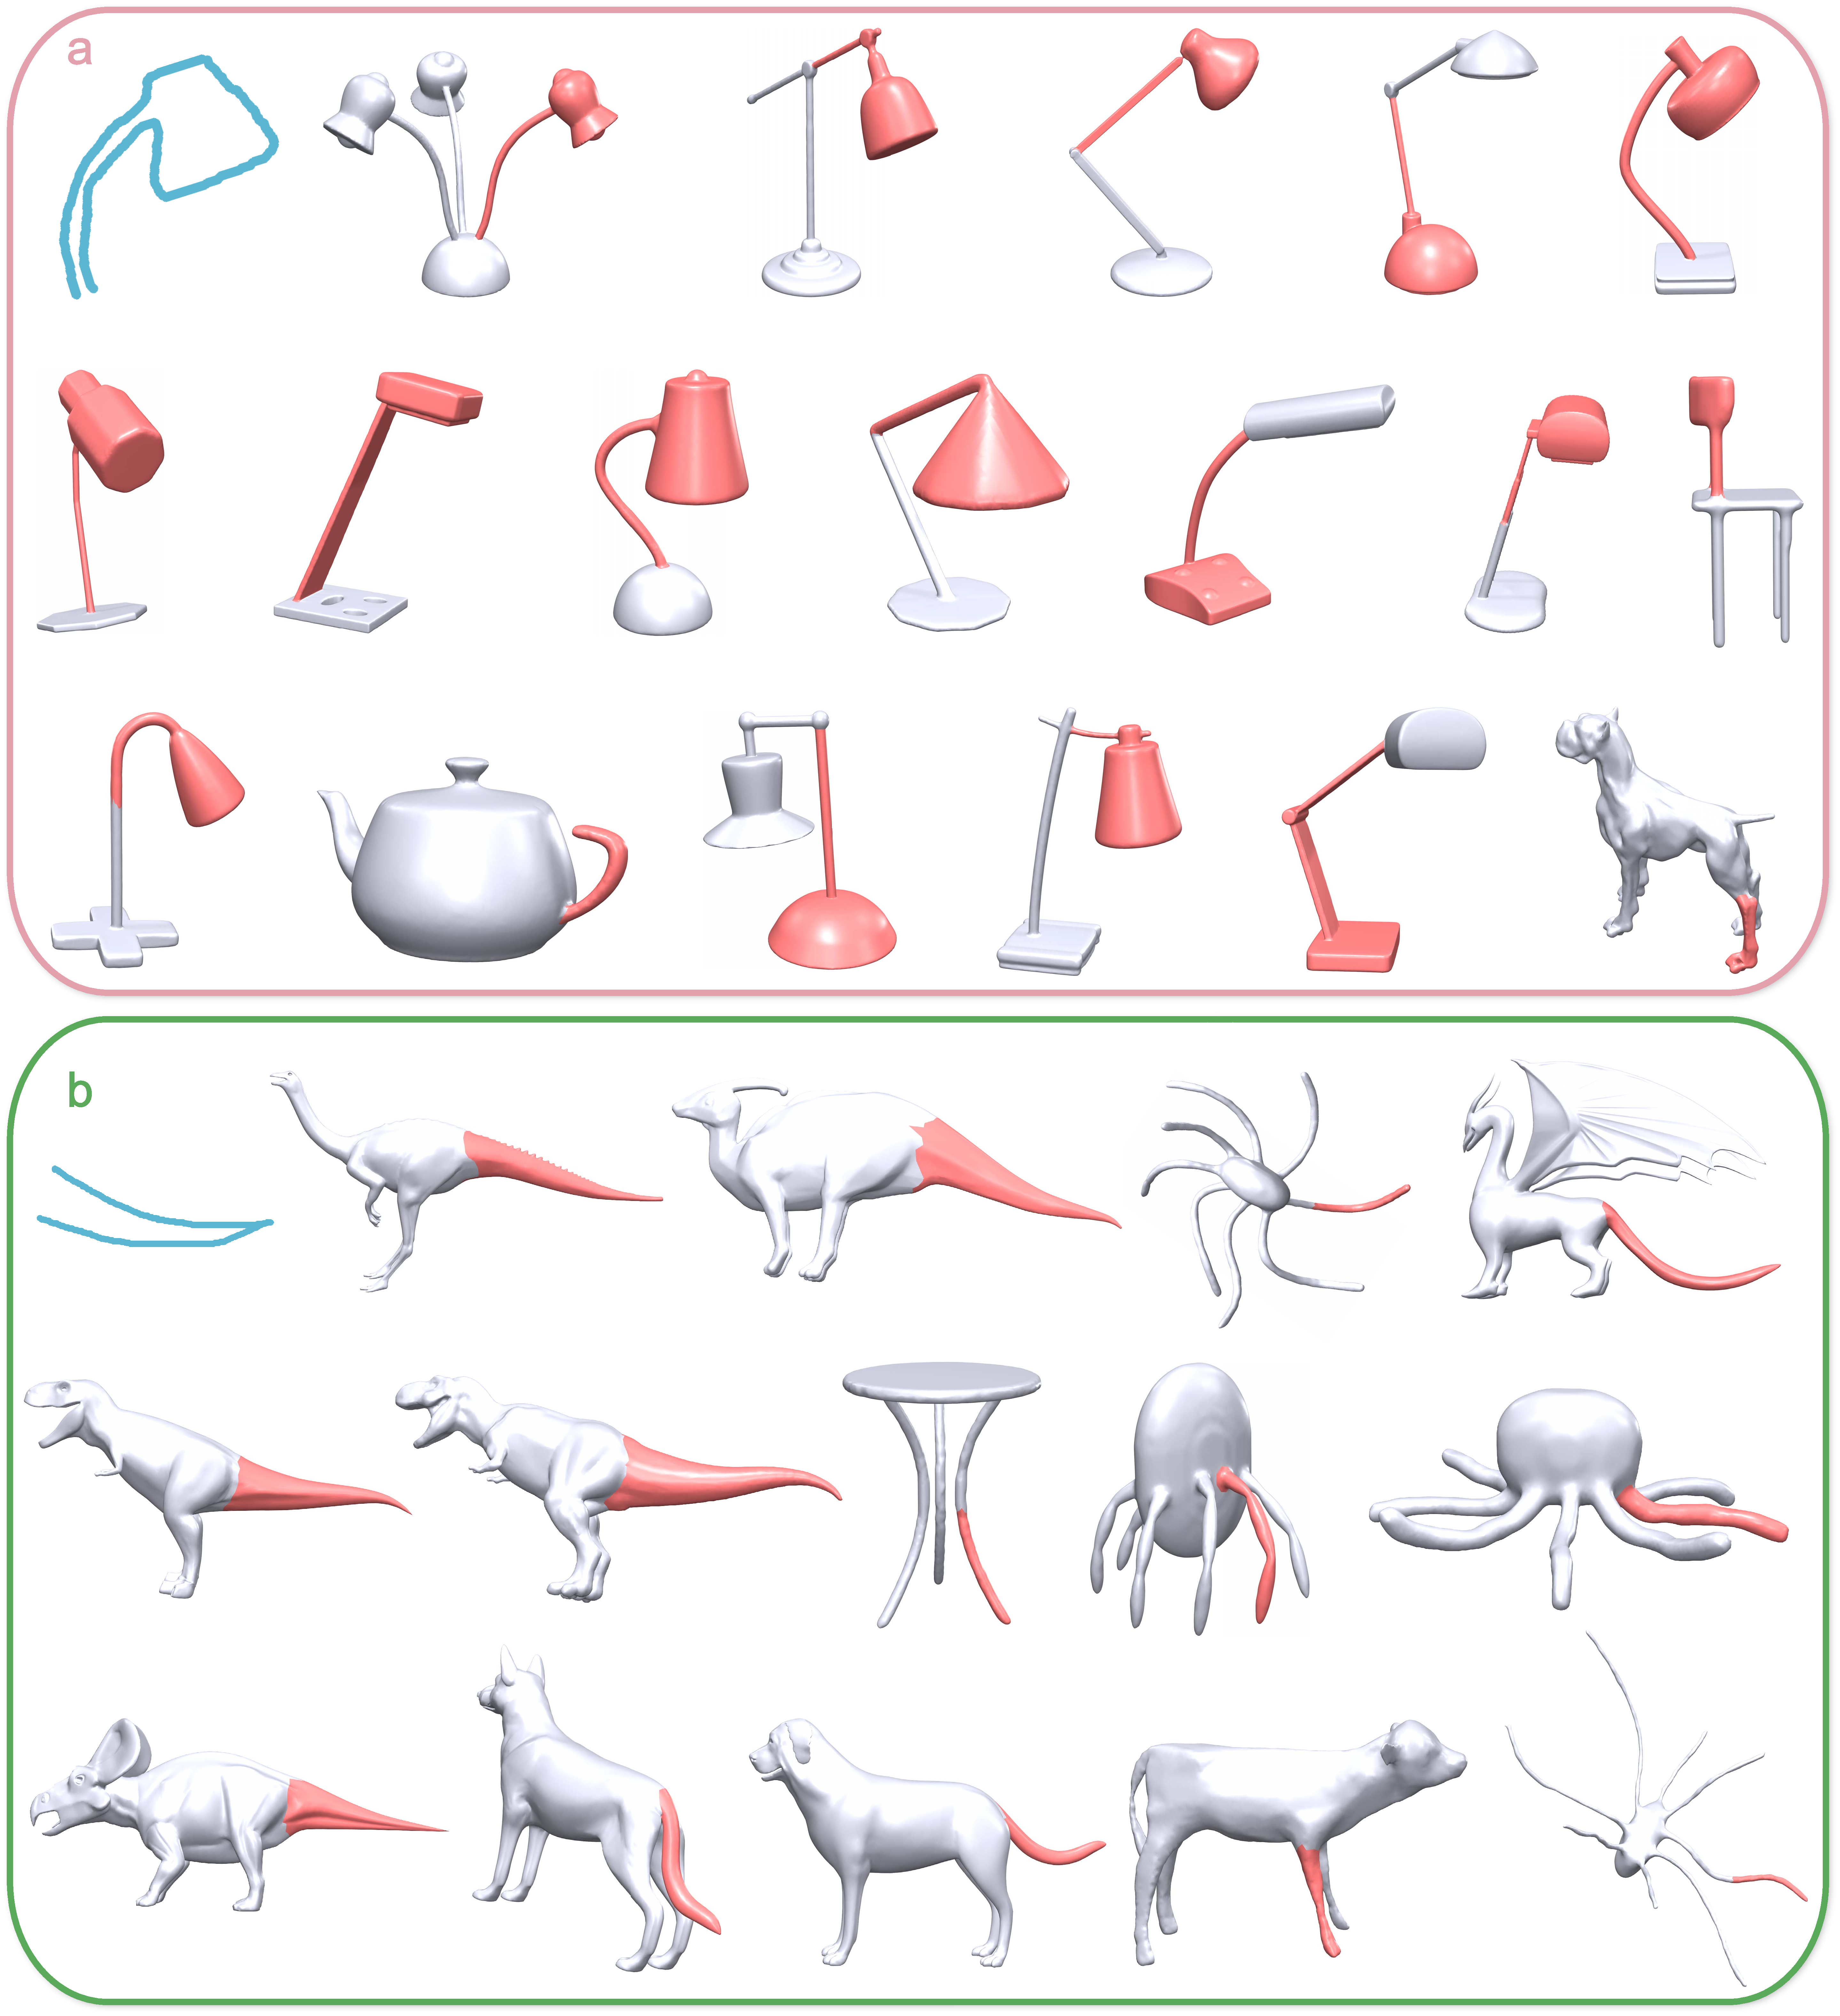
\includegraphics[width=1.05\linewidth]{./Material/MoreRetrievalRes.pdf}
\caption{Retrieval results generated with our method. The retrieved parts are ranked from left to right, form top to bottom.}\label{fig:MoreRetrievalRes}
\end{figure}

There are 513 3D shapes in our database. From these shapes, we extracted 10,773 contours. It took $\sim$3.5 hours to organize these contours into an {\RCKNNG}. The average time to construct the super-face graph of a shape is 20 seconds. Because of the super-face graph representation, our part extraction is real-time. The time for the coarse and fine level extractions for one model is 0.15ms and 10.3ms on average, respectively. Thanks to the two acceleration structures ({\RCKNNG} and SFG) and the coarse-to-fine part extraction strategy, our system can run interactively during the design process. Once a user finishes drawing the sketch, it takes 0.56-0.61 seconds (with GPU and multi-core acceleration) on average for our system to present part suggestions.

\paragraph*{{\RCKNNG} Retrieval Performance.} To evaluate the performance of our {\RCKNNG}, we compare the following methods:
\begin{enumerate}
\setlength{\itemsep}{3pt}
\setlength{\parskip}{0pt}
\setlength{\parsep}{0pt}
\item Traditional (single-layer) $k$NNG constructed by brute force.
\item Wang's randomized $k$NNG approximation~\cite{scalableknnjingwangcvpr2012}.
\item {\RCKNNG} constructed by brute force.
\item {\RCKNNG} with Wang's randomized approximation (\mbox{\textbf{our method}}).
\end{enumerate}
For the two $k$NN graph methods (1 and 2), nodes of the graph are complete shape contours. Node adjacencies and edge weights are identified by global comparison of shape contours. \hl{To compute the contour descriptor of the shape contour, the shape contour is first sampled under 3 different scales. 50, 150, and 250 points along the contour are sampled respectively. The contour descriptor is calculated for the sampled points.} When searching for partial matches to a query contour, we must extract similar contour sections explicitly, significantly slowing down both methods.

For the two {\RCKNNG} methods (3 and 4), nodes of the graph are contour sections (Section \ref{sec:acc}). In our evaluations, we set $k = 20$  and extract $6$ sections from each shape contour.

The retrieval performance for each method is shown in Table \ref{tab:RCKNNGComp}. It is clear that RC-$k$NNG with Wang's method, as proposed in this paper, has the best performance. For retrieval, it is about 97 times faster than Wang's $k$NNG, with only 3 times the construction time. The $k$NNG approaches, which require explicit partial matching at runtime, are much slower.

\hl{We could clearly see the x improvement from Table }\ref{tab:RCKNNGComp}\hl{. The retrieval results generated by the four methods is shown in figure }\ref{fig:RCKNNGComp}\hl{. For the two $k$NNG methods, the retrieved parts are nearly the same. For the two {\RCKNNG} methods, the retrieved parts are nearly the same. But the retrieved parts are different for the two types of the methods.}
%--------------------------
\begin{table}\centering \renewcommand\arraystretch{1.3}
\begin{tabular}{|c|c|c|c|}
\hline \diagbox{Algorithm}{Performance}       & RT  & CT         & ME  \\
\hline BF $k$NNG                     & 4.54s  & 51.7h   & 0.075   \\
\hline Wang $k$NNG                   & 5.68s  & 1.15h   & 0.0795  \\
\hline BF {\RCKNNG}   & 0.053s & 33.89h & 0.07  \\
\hline Wang {\RCKNNG}            & 0.058s & 3.52h  & 0.07  \\
\hline
\end{tabular}
\caption{Retrieval performance for different methods on our test dataset. RT is the retrieval time for a query contour. CT is the construction time for the {\RCKNNG} data structure. ME is the matching error for the retrieval results.
BF $K$NNG represents the Brute force $k$NNG method. Wang $k$NNG represents the Wang's $k$NNG approximation method.
BF {\RCKNNG} represents the {\RCKNNG} with the brute force method.
Wang {\RCKNNG} represents the {\RCKNNG} with Wang's method.}\label{tab:RCKNNGComp}
\end{table}
%--------------------------
\begin{figure} \centering
\includegraphics[width=1.0\linewidth]{./Material/RCKNNGComp.pdf}
\caption{Retrieved parts generated with different methods: the brute force $k$NNG method (a), the Wang's randomized $k$NNG approximation method (b),
the {\RCKNNG} with the brute force method (c), and the {\RCKNNG} with Wang's method (d).}
\label{fig:RCKNNGComp}
\end{figure}
%--------------------------
\begin{figure}\centering
\subfigure[Different methods]{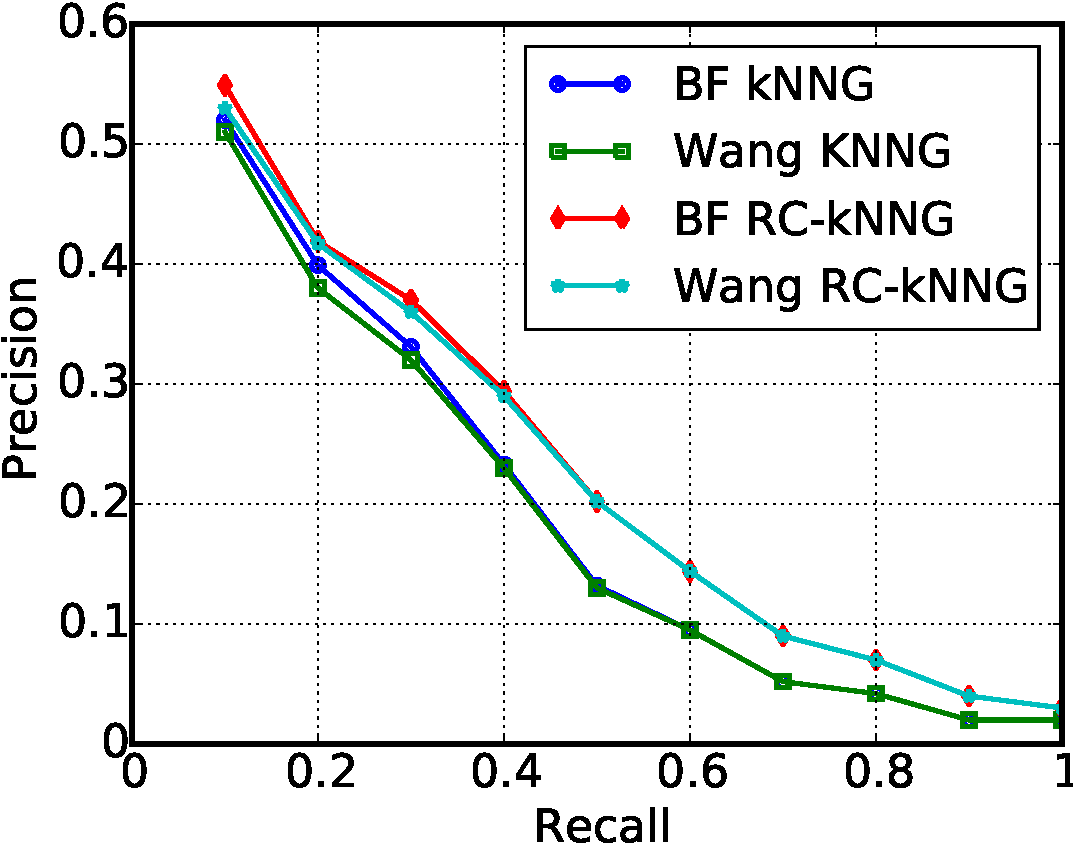
\includegraphics[width=0.49\linewidth]{./Material/PreRecDifAlg.pdf}}
\subfigure[Different camera views]{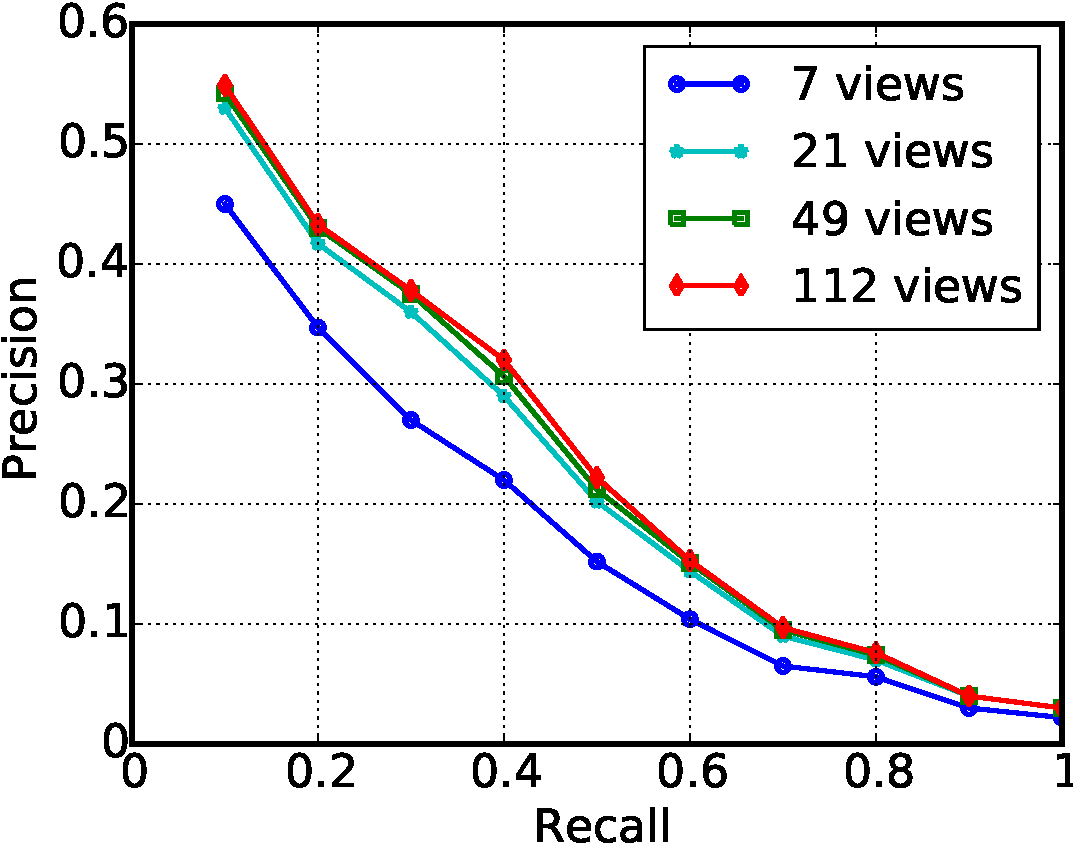
\includegraphics[width=0.49\linewidth]{./Material/PreRecDifViews.pdf}}
\caption{Averaged precision recall curves. (a) compares different retrieval methods. (b) compares different camera views. 
In (a), BF kNNG represents the Brute force $k$NNG method; Wang kNNG represents the Wang's $k$NNG approximation method; 
BF RC-kNNG represents represents the {\RCKNNG} with the brute force method; 
Wang RC-kNNG represents the {\RCKNNG} with Wang's method.}\label{fig:PreRecCurve}
\end{figure}

%--------------------------
\begin{table}\centering \renewcommand\arraystretch{1.3}
\begin{tabular}{|c|c|c|c|}
\hline \diagbox{Step}{SF Count} & 50    & 100    & 200    \\
\hline Construction of SFG      & 20s    & 14.01s  & 19.07s  \\
\hline Coarse extraction (per shape)  & 0.15ms  & 0.77ms   & 3.91ms   \\
\hline Full part extraction    & 560ms  & 577ms  & 605ms  \\
\hline
\end{tabular}
\caption{Timing statistics with different super-face counts. Full part extraction measures the time from launch of a query to generation of a final part.}\label{tab:SFCounts}
\end{table}
%--------------------------

%--------------------------
\begin{table}\centering \renewcommand\arraystretch{1.3}
\begin{tabular}{|c|c|c|c|}
\hline \diagbox{}{SF Count} & 50    & 100    & 200    \\
\hline Matching error      & 0.45     & 0.29   & 0.07   \\
\hline
\end{tabular}
\caption{Matching error statistics with different super-face counts, averaged over a set of 20 test sketches.}\label{tab:MatchError}
\end{table}
%--------------------------

\paragraph*{Increasing Super-Face Counts.} In Table \ref{tab:SFCounts}, we show the timing statistics for different super-face counts. The coarse-level part extraction time is strongly dependent on the number of super-faces. However, this is a relatively fast step so this dependence does not significantly hurt overall performance. Overall, despite quadrupling the number of super-faces, part extraction remains interactive, completing in well under 1s.

In Figure \ref{fig:SFCountsPartQuality}, we show the qualitative improvement in part extraction as we increase the number of super-faces. With fewer super-faces, the search space is relatively coarse and the extracted parts need not perfectly match the sketch. As we increase the number of super-faces, the search space becomes more fine-grained. The part contours match the sketch better and better, and the part boundaries are less constrained to follow suboptimal cuts. We quantitatively evaluate the quality of the extracted part by comparing the contour of the extracted part with the user's sketch in terms of the contour descriptor introduced in Section \ref{subsec:CtourDesc}. Table \ref{tab:MatchError} shows the matching error statistics for different super-face counts. Note that the error decreases substantially as the shape representation becomes more fine-grained.

\begin{figure}[h!] \centering
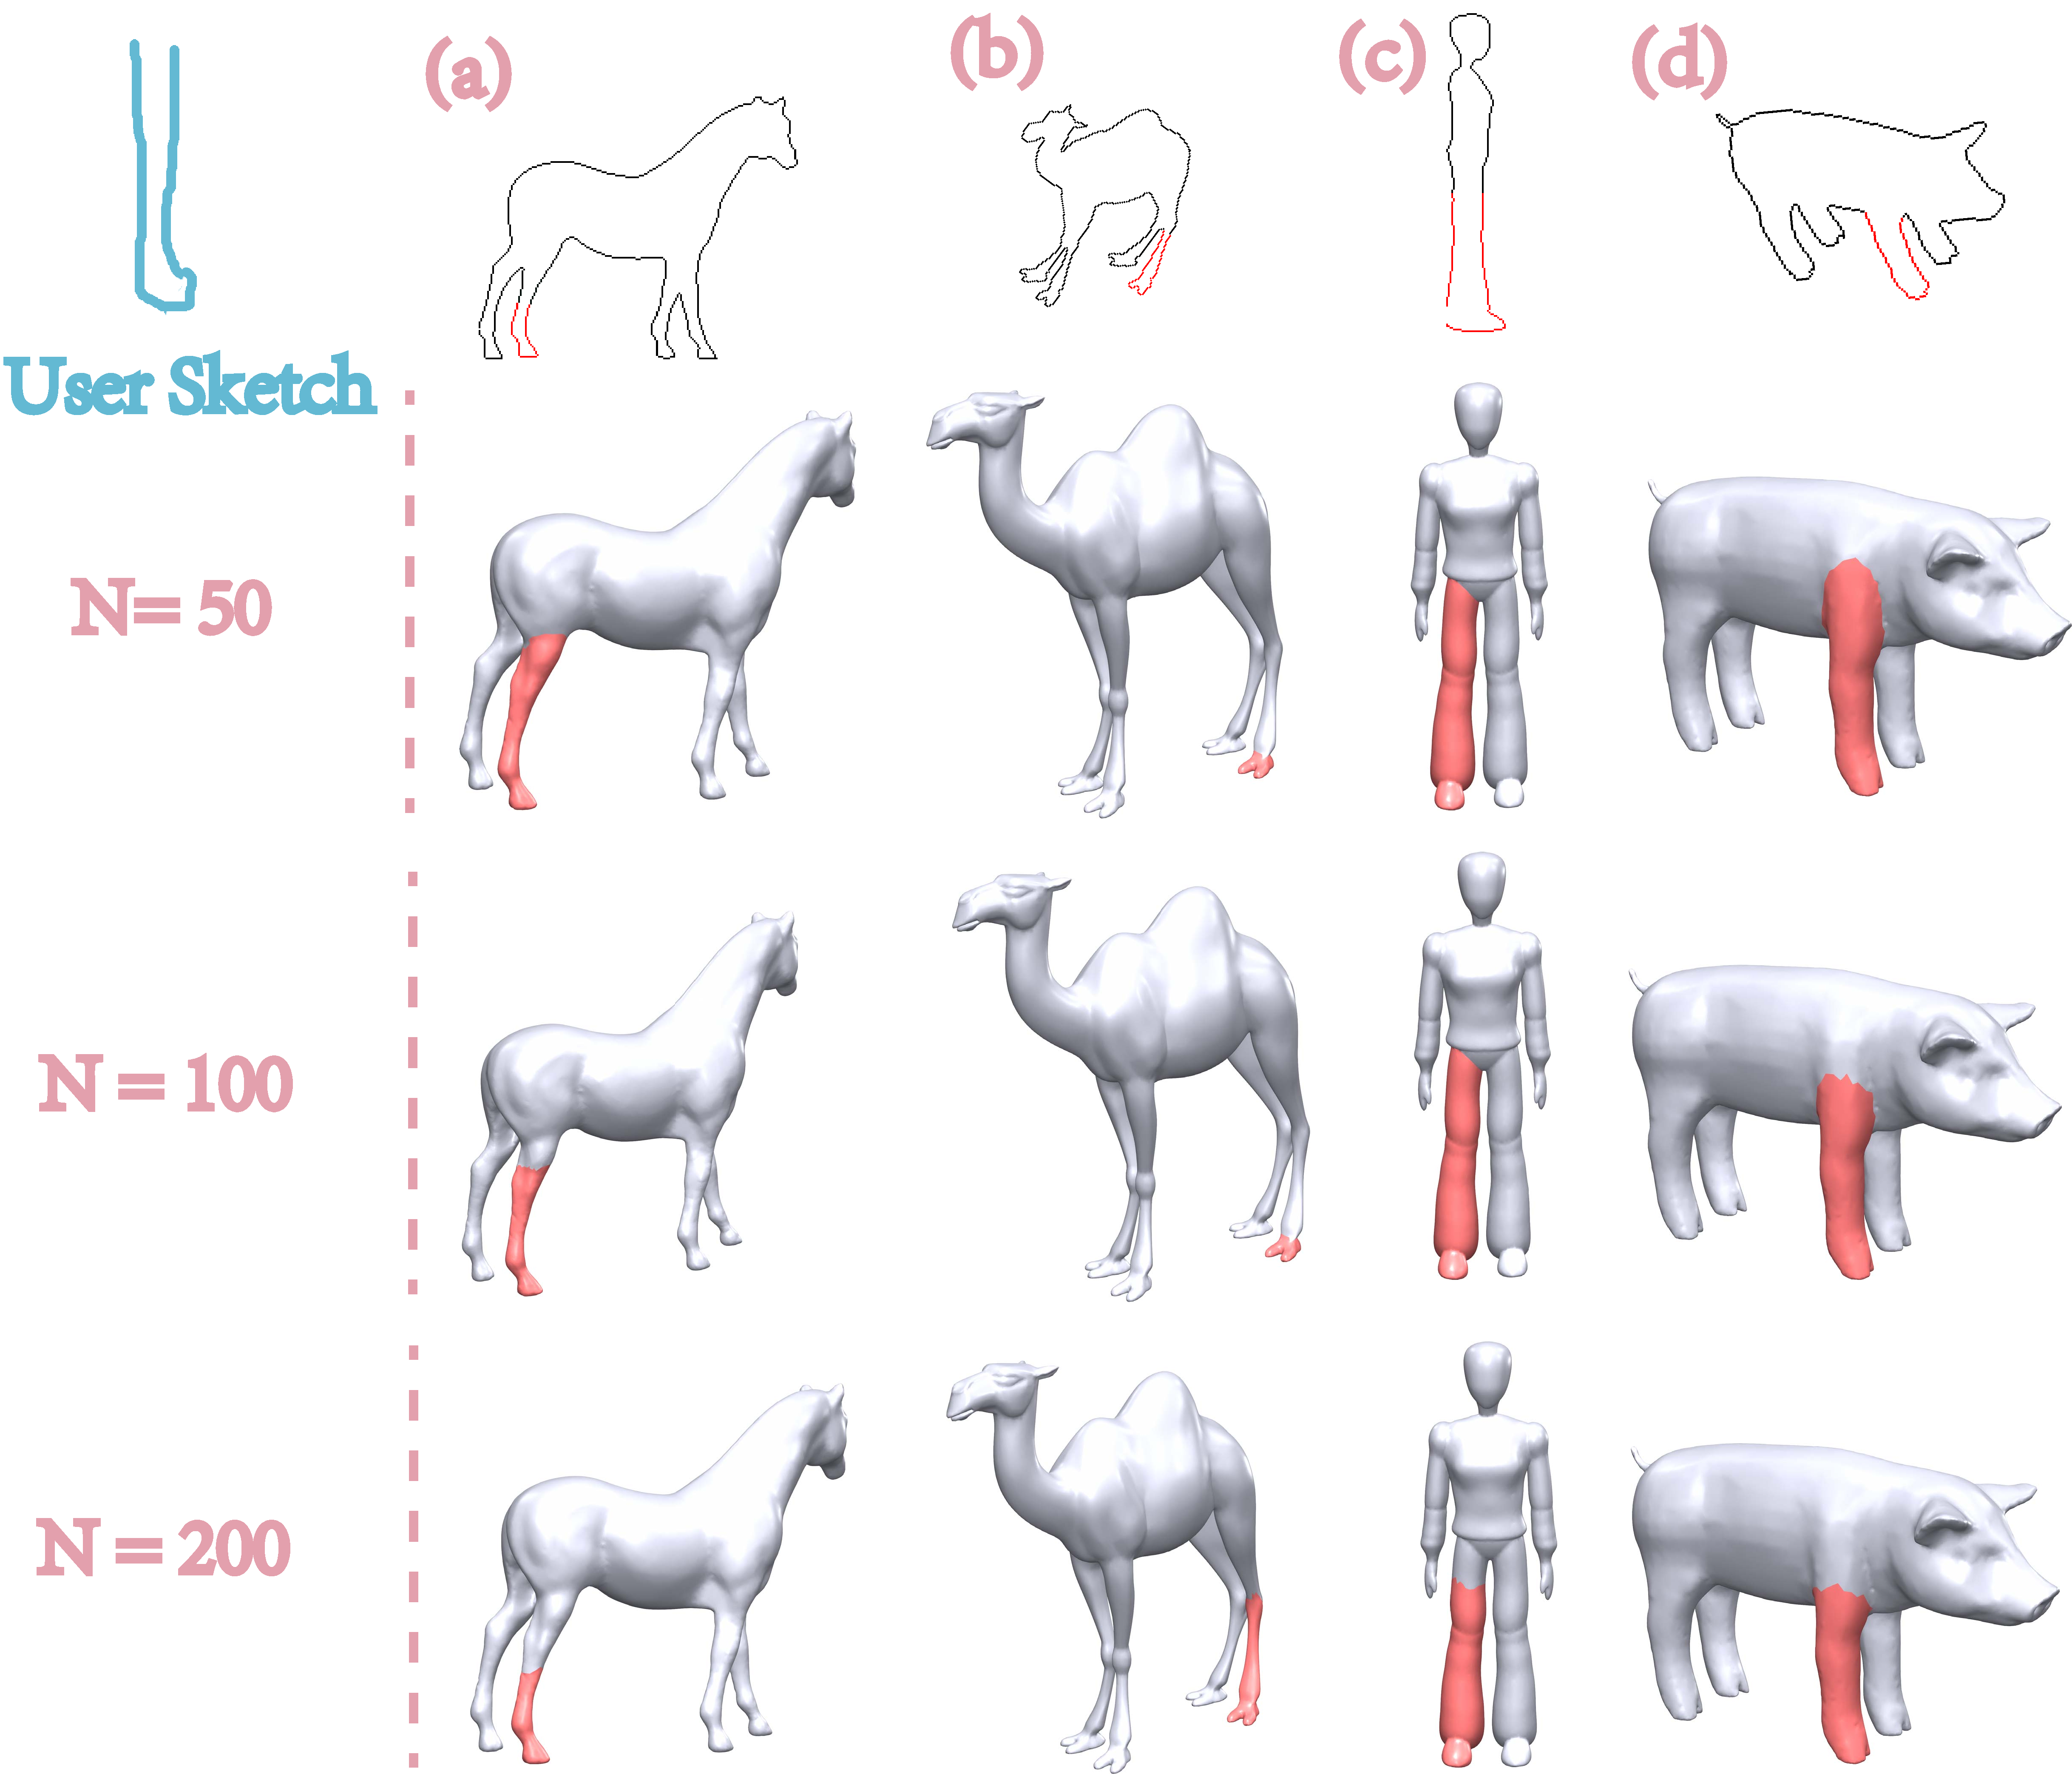
\includegraphics[width=1.0\linewidth]{./Material/SFGNVary.pdf}
\caption{Improvement in part quality with increasing super-face count (N). With more super-faces, the extracted part fits the user's sketch better and better.}
\label{fig:SFCountsPartQuality}
\end{figure}

\paragraph*{Comparison.}\hl{ We compare our method to the approach depending on the presegmented database (PreSeg). The PreSeg method is performed as follows: 1). Each database model is pre-segmented into regular (typical semantic) parts. For example, a human model is decomposed into four parts: head, torso, arms, and legs. 2). We extract boundary contours for each part under different camera views. 3). We construct the kNN graph for the part contours. The node in the kNN graph represents the complete part contour. The edge is established by global matching between part contours. 3). In the runtime stage, given the 3D proxy, a list of candidate parts are retrieved through a similar procedure as Ours with the only difference that contour matching is performed in a global manner. The matching error for the PreSeg method is 0.624 averaged over a set of 20 test sketches. Compared with Table }\ref{tab:MatchError}\hl{, our method clearly outperforms the PreSeg method. The visual result is shown in figure }\ref{fig:Comp2PreSeg}\hl{. Because our method generate candidate parts on-the-fly, the retrieved parts are more similar to the user sketch.}
%--------------------------
\begin{figure}\centering
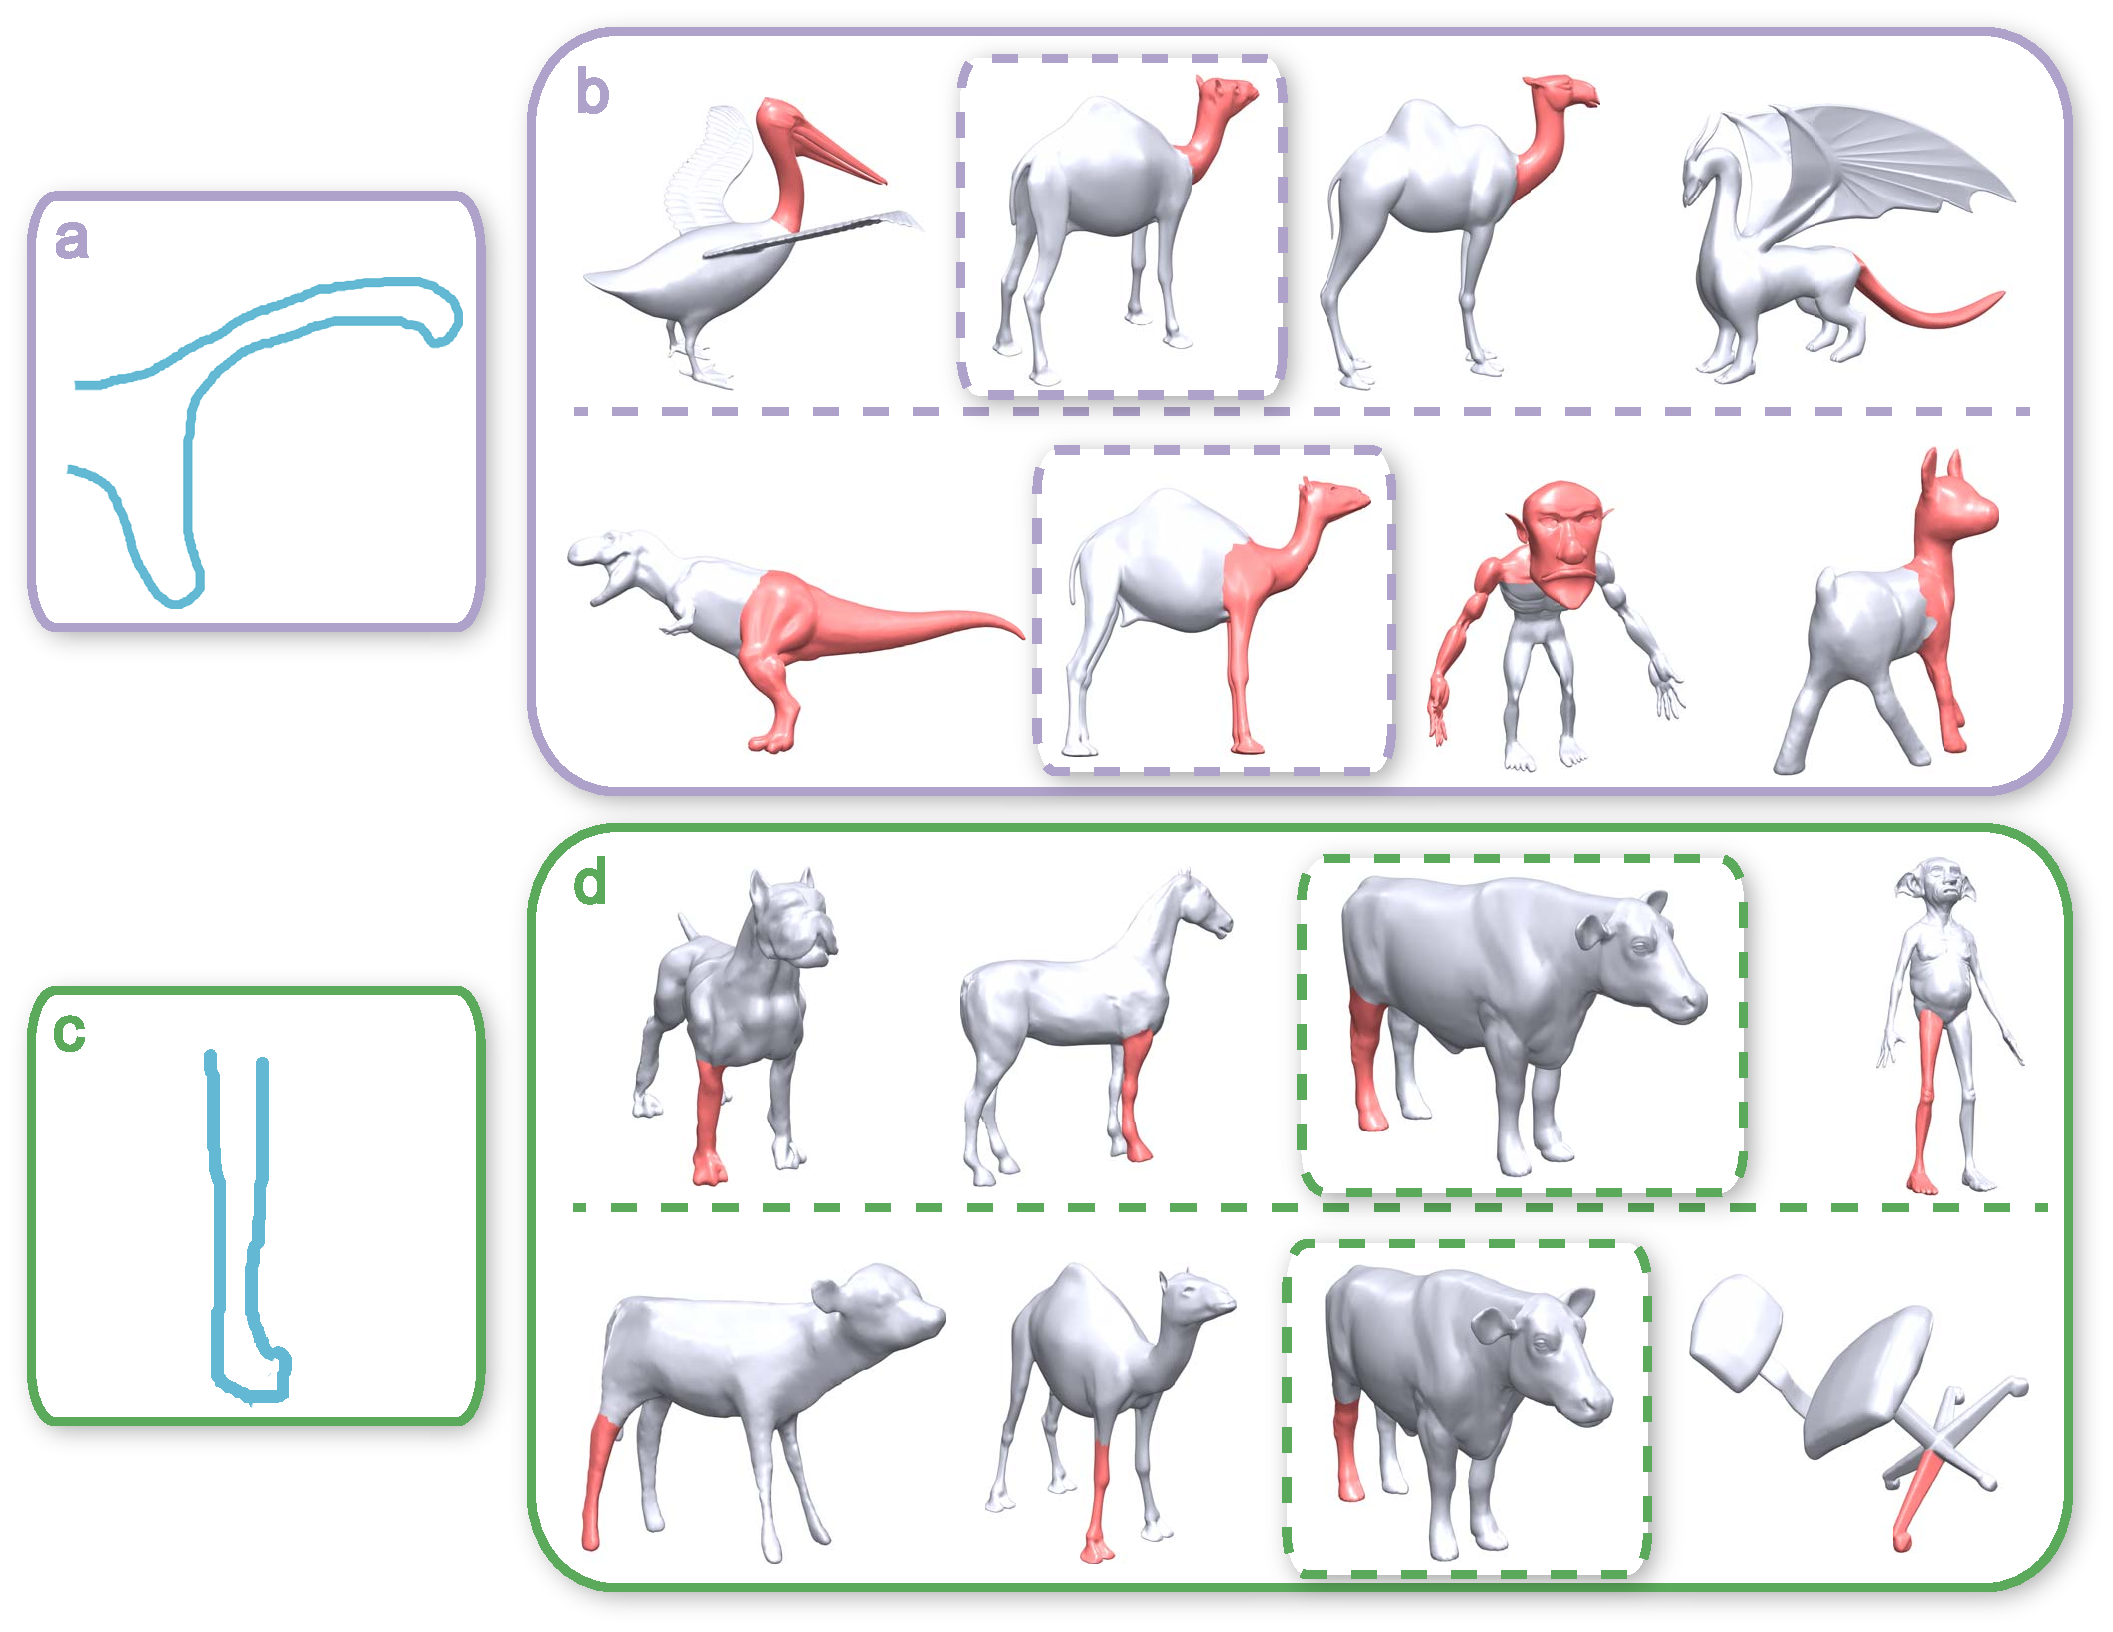
\includegraphics[width=1.0\linewidth]{./Material/Comp2PreSeg.pdf}
\caption{Retrieval results generate with our method and PreSeg method. Given the same sketch, we show the retrieval results generated with the two methods.
In (b) and (d), our results is on the upper row, the PreSeg results is on the lower row. Notice the results circled in (b) and (d), we could conclude that our method could generate candidate parts more similar to the user sketch.}\label{fig:Comp2PreSeg}
\end{figure}

\paragraph*{Camera views.} \hl{We have evaluated the influence of the camera views. Figure }\ref{fig:PreRecCurve}\hl{(b) shows the precision recall curve under different camera views. The 7 camera views include 3 canonical side views and 4 corner views. The other camera views include the 7 camera views and other uniformly sampled views}~\cite{FanWang2013}\hl{. To balance between efficiency and effectiveness, we use 21 views.} 